\newpage
\thispagestyle{empty}
\chapter{Quantum Walks with Time-Dependent Hamiltonians}
The main purpose of this thesis is to study quantum walks with time dependent hamiltonians, focusing in particular on their application to the spatial search problem on graph. The general idea is trying to improve a time-independent implementation of quantum walks search using a time-dependent hamiltonian analogous to the one used in the adiabatic evolution. In order to determine whether this new approach produces successfull results we study two selected graph topology: the circular graph, for which the time-independent approach is not able to solve the search problem, and the complete graph for which the search problem is solved for both the time-independent and adiabatic evolution approaches. \\ We compare the two methods for the optimized-search, localization - which represents a search without needs to optimize the time - and a measure of robustness. 

\section{Search with Time-Dependent Hamiltonian}

    \subsection{Time-Dependent Quantum Walk}
        Following the adiabatic evolution discussed in the preliminaries, we consider a search hamiltonian consisting in an oracle term and a laplacian term, such that at the beginning of the evolution we hamiltonian is equal to the laplacian, while at the end it's equal to the oracle hamiltonian. Such hamiltonian is constructed in the following way:
          \begin{equation}
            H = (1-s(t))L - s(t)\beta|w\rangle\langle w|
          \end{equation}
        where $|w\rangle$ represents the target of the search.
        The function $s(t)$ (referred as \textit{step function}) regulates the evolution of the hamiltonian an plays a  crucial role in the final search probability, as we will later see. It is defined in the following way
          \begin{equation}
            s: [0,T] \rightarrow [0,1]
          \end{equation}
        where T is the time at which the solution is found (or actually, the time that the system is made to evolve. A solution might not be found at such time, or at least found with low probability).


    \subsection{Comments on the shape of s(t)}
        As we mentioned previously the step function s(t) plays a crucial role in the evolution of the system. The classical adiabatic evolution by Farhi et al. \cite{Farhi2000} consists in a linear step function s(t) defined as $s(t) = \frac{t}{T}$, such that the systems evolves linearly. \\


        We however investigate which is the optimal shape of s(t) for otpimal probability. We first consider, somewhat naively, the square root and the cubic root of t/T, and the square and third power of t/T. However, for the complete graph Ronald \& Cerf propose that the optimal shape of s(t) comes from considerations on the separation of the first two eigenvalues \cite{Roland2002}; in particular s(t) should be steeper for larger separation and flatter for small eigenvalues separation. This in indeed somewhat to be expected, considering that for the adiabatic theorem to hold the adiabatic time needs to have a certain value which dependes directly from the eigenvalues separation. \\
        Following that approach we consider a similar step function that tries to emulate the one from Ronald \& Cerf. For this paricular reason we will refer to this particular step function as the Ronald-Cerf s(t) even though it's not exacly the same one they derived. \\


        Follows here a summary of all the step functions considered in the analysis of the circular graph. Note that for the complete graph, since the solution is derived analitically such different s(t) are not considered nor of particular interest.
          \begin{itemize}
            \item \textbf{lin}: $s(t) = \frac{t}{T}$
            \item \textbf{sqrt}: $s(t) = \sqrt{\frac{t}{T}}$
            \item \textbf{Ronald-Cerf(3)}: $s(t) = \frac{1}{2}(2(x-1)^{3}+1)^2$
            \item \textbf{Ronald-Cerf(5)}: $s(t) = \frac{1}{2}(2(x-1)^{5}+1)^2$
          \end{itemize}
        For the Ronald-Cerf step function we considered different values of odd-k, $k=3,5,7$. It is clear that we need to include a picture of the different functions considered and the eigenvalues separation picture for a particular case.

    \subsection{Methods and Dynamics}
        The time evolution operator follows from the time-ordering approach, namely:
          \begin{equation}
            S(t,t_0) = T exp \frac{1}{i\hbar}\Big\{ \int_{t_0}^{t} dt' H(t')\Big\}
          \end{equation}
        where T is the time-ordering.

        \noindent
        In order to find the evolved state we can proceed in the following ways:
        \begin{itemize}
          \item \textbf{Solve the Schroedinger differential equation}
        \end{itemize}
        Since we're only interested in finding the evolved state, having the exact form of the evolution operator is somewhat irrelevant. Focusing our attention on the solution of the differential equations also helps us from a computational point of view; indeed the implementation of the differential equation solver is much simpler than any of the other two possibilities.

            \subsubsection*{Solving the Schroedinger Equation}
            From the intial state $|\psi\rangle$ we're intested in finding the evolved state $|\psi(t)\rangle$, and we proceed solving the differential Schroedinger equation:
              \begin{equation}
                i\frac{d}{dt}|\psi(t)\rangle = H |\psi(t)\rangle
              \end{equation}
            Since H is a matrix we had to solve it for components. Recalling that $|\psi\rangle$ is a vector in an N-dimensional Hilbert space, we need to solve N-differential equations of the form:

              \begin{equation}
              \frac{d}{dt}|\psi_i(t)\rangle = \sum_jH_{ij}|\psi_i(t)\rangle
              \end{equation}
            We also need to impose boundary conditions, namely that $|\psi(0)\rangle = |\psi\rangle$, our initial ground state.

        \subsection{Multiple Runs for One Search}
        To give a complete picture of the usefulness of the time-depedent approach, we consider the possibility of repeating the search multiple times. If the probability at which the solution is found is $p=1$ the search is perfect and the problem is solved. However, if the proabability is less than one, i.e. imperfect search, the problem can be solved by searching multiple times . Since the results of the search are checked independently, a single successfull search is sufficient, and this kind of routine is efficient as long as the probability $\big|\langle\psi(t_f)| w\rangle\big|^2$ is greater than $1/poly(N)$ (where N is the dimension of the graph) \cite{Morley2018}.

        Repeating the search multiple times does however come at a cost. It is indeed necessary to take into account for a non-zero \textit{initialization} time $t_{init}$ to prepare the system in the correct state as well a physical time for the measurement. Therefore, computing multiple searches with small $t_f$ becomes less efficient than less searches with larger $t_f$, where the quantity $t_{init}$ makes a lesser contribution to the overall $t_f$. Clearly this consideration is particularly relevant for increasing graph size.

\section{Selected Topology: Circular and Complete Graph}
    Throughout our analysis we will focus the attention on two selected graph topology, the ring graph (R) and the complete graph (C). \\

    As previously discussed in Section? the \textbf{complete graph} represents the best case scenario since it has been shown to solve the search problem both for the standard time-independent quantum walk approach and the local adiabatic evolution, with a speed up of $\sqrt{N}$. An adiabatic implementation -where with adiabatic we consider the time-dependent approach with additional adiabatic-theorem conditions -  of the quantum walk search does not work with the usual Grover's oracle requiring a more elaborate structure, however as we shall later see a merely time-dependent approach might be somewhat interesting. \\

    The \textbf{circular graph} on the other hand is not able to solve the search problem with the time-independent approach, and can give some interesting insights with the application of the time-dependent quantum walk search.  \\

    The choice of graph topology is therefore based on the idea of giving results at either side of the spectrum of 2-dimensional graphs, trying to improve a non-working approach on one side, and get some interesting insights on an already perfect-search approach on the other.

\section{Characterization of the results: Search, Localization and Robustness}
    \subsection{Search vs Localization}
      Before looking at the results it's necessary to characterize two particular classes of results, the \textbf{search} and the \textbf{localization}, that help us decide whether the time-dependent approach does bring any advantages.
      \begin{itemize}
          \item the (optimized) \textbf{search} describes the usual search, namely the finding of the solution with high probability (possibly unitary) for the smallest time as possible. As previously mentioned we also take into account the possibility of repeating the search multiple times.
          \item the \textbf{localization} describes the finding of the solution with high probablity without the need to optimize the time. This description becomes necessary if we take into account the adiabatic nature of the time-dependent approach, that guarantees unitary probability for large enough $t_f$.
      \end{itemize}

    \subsection{Robustness}
        We've seen that the probability of a search problem depends on the time $t_f$ at which the quantum state is measured and the parameter $\gamma$. The optimal probability, i.e. highest possible, clearly is given by the optimal combination $t_f-\gamma$, and since the time $t_f$ should not be bound to errors give it's the time at which the state is measured, fluctuations in the probability are necessarily caused by fluctuations in the $\gamma$ parameter. \\
        Following from \cite{SH.HungS.Hietala2019} we define the \textbf{robustness} as quantitative measure representing the variation on the probability due to some perturbation/noise on $\gamma$.
        We begin by finding the optimal probability $P$, evaluated with the single or multiple run for one search approach. For the corresponding $(t_f,\gamma)$ combination we evaluate the robustness as follows:
        \begin{equation}
            R ^\pm = P(t_f, \gamma) - P(t_f, \gamma \pm \delta)
        \end{equation}
        where $\delta$ is some positive perturbation of the $\gamma$ parameter. As we shall later see this quantity is given in terms of some percentage of $\gamma$. To find a unique value for the robustness an average of $R^\pm$ is done:
        \begin{equation}
            R = \frac{R^++ R^-}{2}
        \end{equation}
        The quantity R should be positive, since the $(t_f,\gamma)$ combination should produce the highest probability possible. We also that the perturbation on the parameter has equal probability of being positive or negative, thus the average ponderates between these two possibilities. \\ \\It is necessary however to remember that the value $R$ does not have any absolute physical significance, but fits well for our specific scenario where the interest is focused on the comparison between two specific approaches. Therefore this quantity will be solely used to characterize a particular approach as \textbf{more} or \textbf{less robust}.

\section{Results for the Circular Graph}

    \subsection{Time-Independent Benchmarks}
        The first step of the analysis is to compute time-independent benchmarks. We computed the probability over a time-beta grid, with $T\in[0,N]$ and $\beta\in[0,2.5]$, where N is the dimension of the graph considered. An initial run of the probability distribution showed that \textit{it is worse than linear in T}, thus the need to see times greater than $T=N$ proved to be unnecessary. In addition Grover algorithm for the unstructured search (and the complete graph) goes like $\sqrt{N}$ and the adiabatic (globally, not locally) goes like $N$, thus focusing on $T \leq N$ made much more sense. \textbf{It's interesting to show a figure with the probability distribution for some sampled $\beta$ even for large time, giving the idea that the probability does indeed not increase with time and we can focus the attention to smaller T (T<N)}.
        Throughout the analysis we will consider graphs up to N = 71, with only odd dimensions which makes a easier oracle placement (hamiltonian is somewhat symmetric). Additional considerations and reasoning for the time-beta grid can be found in Appendix A. \\


        To display the results in an intuitive way we used a heatmap plot, which gives a good idea on the probability distribution for varying combinations of $(T,\beta)$:

          \begin{figure}[ht]
            \centering
            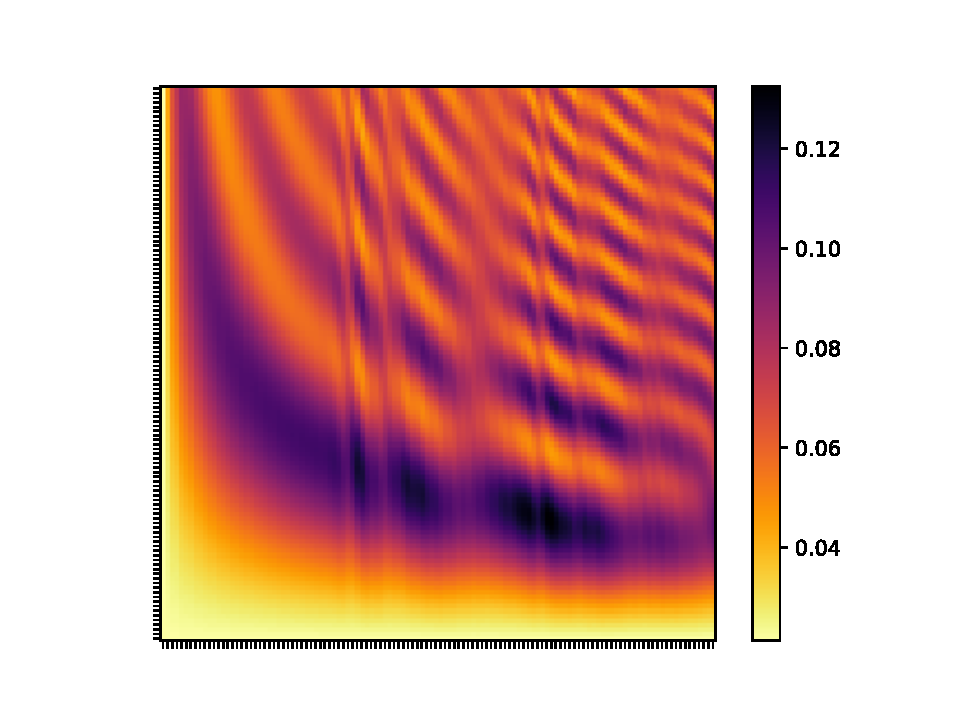
\includegraphics[width=9cm]{./figures/time_independent_benchmark_47}%
            \caption[Probability heatmap plot for the time-independent hamiltonian, N=47]{\textbf{Probability heatmap plot for the time-independent hamiltonian.} The figure shows the probability distribution for a circular graph of N=47 simulated using the time-independent hamiltonian, providing thus the necessary benchmark. Note that darker color do not represent probabilities close to one, but only higher probability regions.}
          \end{figure}

        \subsubsection*{Comments on the probability distribution}
        It is quickly noticeable that the probability distribution is not smooth, indeed it shows peaks (darker regions) and valleys (lighter regions). This is both present for fixed $\beta$, i.e. any orizontal line, and for fixed time, i.e. any vertical section considered. We will later see that this is somewhat a weakness of the time-independent approach, since a small variation of the parameter $\beta$, which reperesents as previosly mentioned the deepness of the well or an energy parameter, leads to possibly great variation of the probability. We shall call this fenomena \textbf{non-robustness}.

    \subsection{Time-Dependent Results}
        Similarly we computed the grid probability using the time-dependent hamiltonian previously introduced. To easily comparing the two methods we opted to consider the same time $T=N$, and from an initial run we discovered that the $\gamma$ parameter affected similarly the probability, namely the probability tended to be higher for smaller values of $\gamma$, thus we used approximately the same range. \\

        The simulation is then run for all the step functions $s(t)$ previsouly discussed, and an intuitive heatmap plot is outputted.
        \begin{figure}[ht]
        \centering
        \begin{tabular}{cc}
          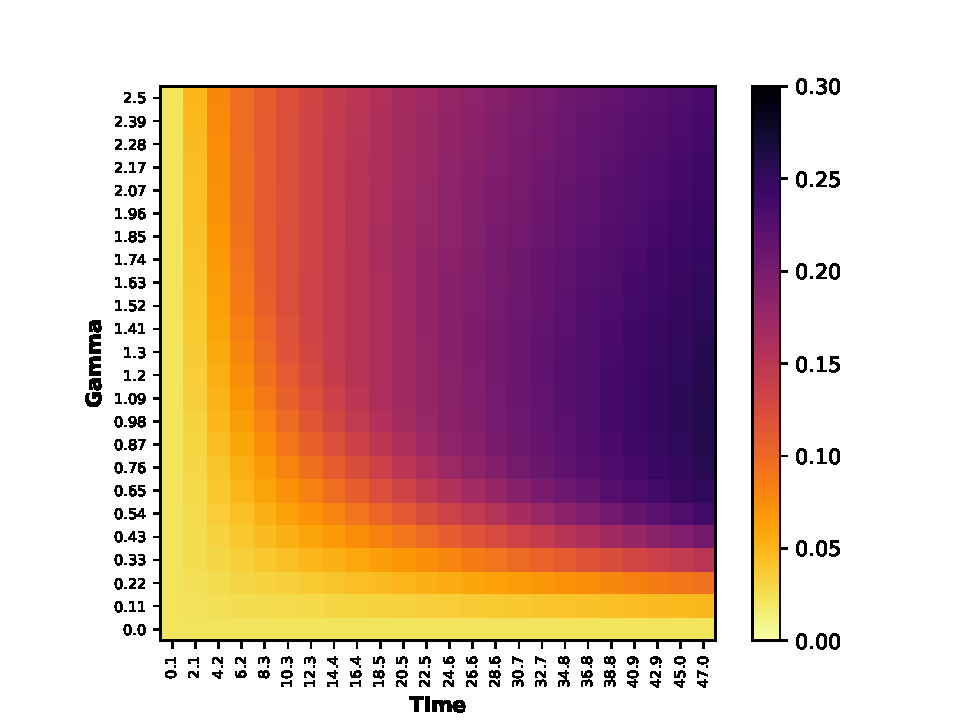
\includegraphics[width=75mm]{./figures/time_dependent_heatmap/47_heatmap_time_dependent_lin.pdf} &   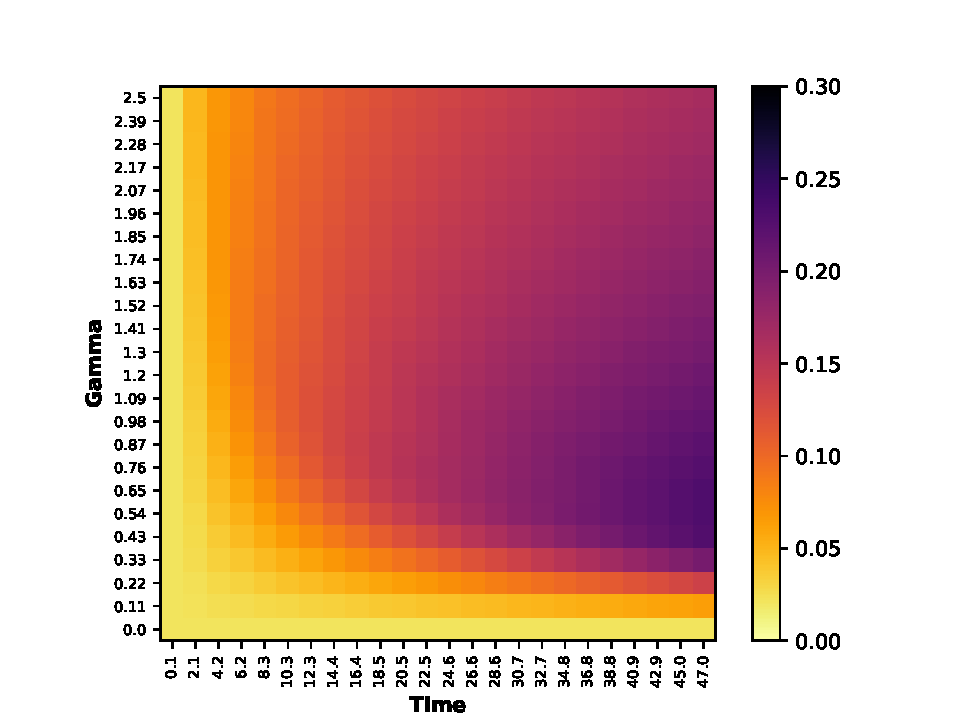
\includegraphics[width=75mm]{./figures/time_dependent_heatmap/47_heatmap_time_dependent_sqrt.pdf} \\
        (a) lin & (b) sqrt\\[6pt]
        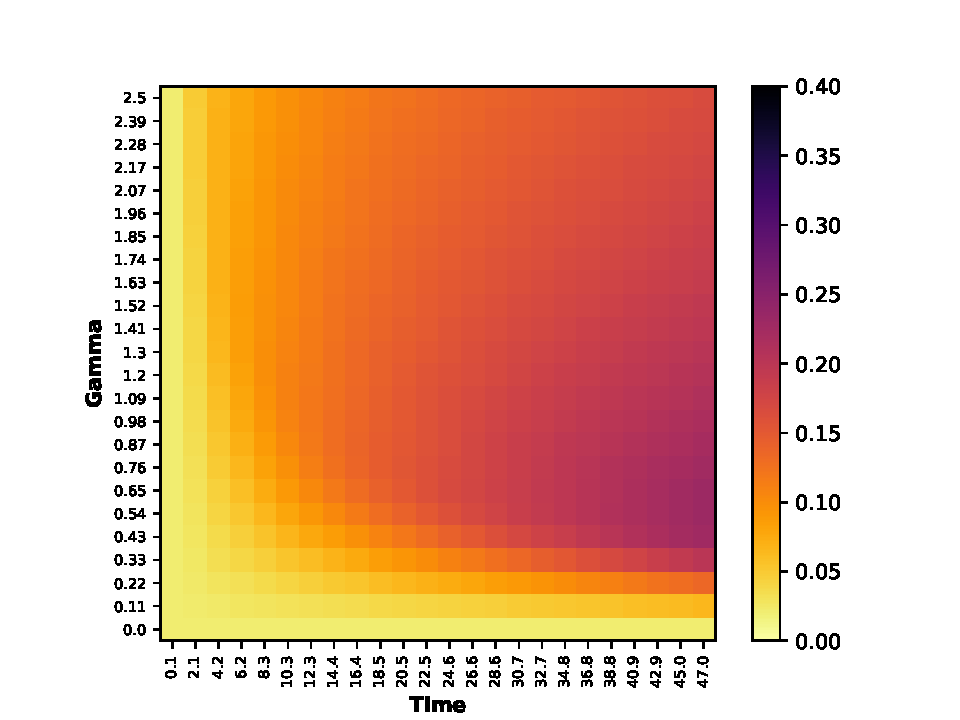
\includegraphics[width=75mm]{./figures/time_dependent_heatmap/47_heatmap_time_dependent_cbrt.pdf} &   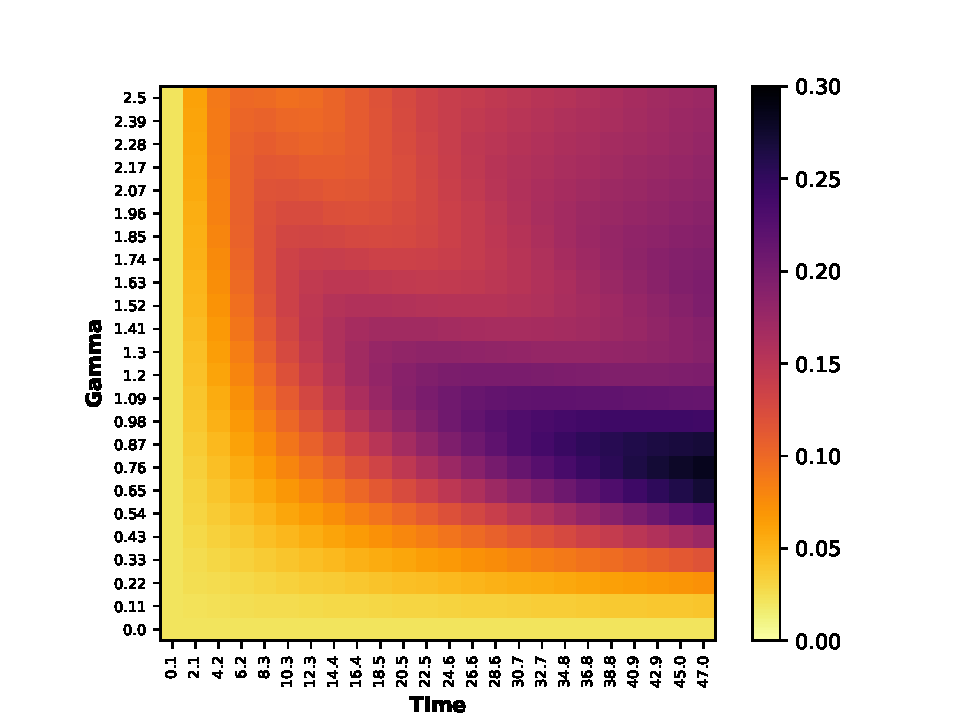
\includegraphics[width=75mm]{./figures/time_dependent_heatmap/47_heatmap_time_dependent_cerf.pdf} \\
        (c) cbrt & (d) cerf\\[6pt]
        \end{tabular}
        \caption[Probability heatmap plot for the time-dependent hamiltonian, for different shapes of s(t)]{\textbf{Probability heatmap plot for the time-dependent hamiltonian, for different shapes of s(t).} The figure shows the probability distribution for a circular graph of N=47 evaluated using the time-dependent hamiltonian using the following step functions (a) linear, (b) $\sqrt{t/T}$, (c) $\sqrt[3]{t/T}$ and (d) Ronald-Cerf(3). Note that the probability gradient is normalized to p=0.3 to accentuate the difference in probability between different regions. }
        \end{figure}

        \subsubsection*{Comments on the probability distribution}
        \clearpage

    \subsection{Comparison: Localization}
        We now compare the localization properties of the two algorithm. As we mentioned in the comments to the probability distributions of the time-independent and time-dependent approaches we discovered the following:
        \begin{itemize}
            \item \textbf{Time-Independent QW}: the time-independent based search is not able to solve the search problem with a single iterations, thus making it necessary to run multiple searches. This implies that the approach does not show any localization properties, in fact the probability does not increase with time as in the time-dependent approach.
            \item \textbf{Time-Dependent QW}: the time-dependent based search on the other hand because of the adiabatic theorem does solve the search problem with a single iterations, although that happens for fairly large $t_f$.
        \end{itemize}
        Although the time-dependent approach is able to get to unitary probability in a fairly large $t_f$, it is able to produce large enough probabilities in much less time, as we can see from this plot. This is a consequence of the fact that the probability does not grow linearly with time, thus needing larger $t_f$ closer it gets to $P=1$. \textbf{include plot}


    \subsection{Comparison: Search}
        In order to compare the two approaches for the search it is clear that we cannot simply consider the time at which the solution is found with unitary probability, since that particular $t_f$ is not optimized for the time-dependent approach and does not exist for the time-independent one. Therefore, as previously mentioned we consider the possibility of doing multiple runs for one search. For this reason we introduce the following quantity
        \begin{equation}
          \min\Big(\frac{t_f}{p}\Big)
        \end{equation}
        where $1/p$ is the number of iterations necessary to get to unitary probability (statistically), and combining it with $t_f$ gives the total time necessary. Optimizing over the combination of $t_f$ and $p$ gives the smallest time necessary to get to unitary probability using the multiple search approach. Additionally, the number of iterations $\mbox{iters}=1/P$ might give some useful insights on the performance of the approach, in particular if you take into account the initialization time $t_{init}$\\ \\  However, this particualar approach poses a few problems. Infact if we look at how the quantity $t_f/p$ varies for varying $t_f$, we discover that the minimum of such quantity will always be for the smallest $t_f$ available, regardless of the type of hamiltonian and step function $s(t)$. The following plot does indeed show, for a few sampled $\gamma$, the shape of $t_f/p$. In addition, in Section ? we mentioned that when dealing with multiple runs for one search we need to take into account an initialization time $t_{init}$. It is thus necessary to consider a lower bound on $t_f$.
        \begin{figure}[ht]
        \centering
        \begin{tabular}{cc}
          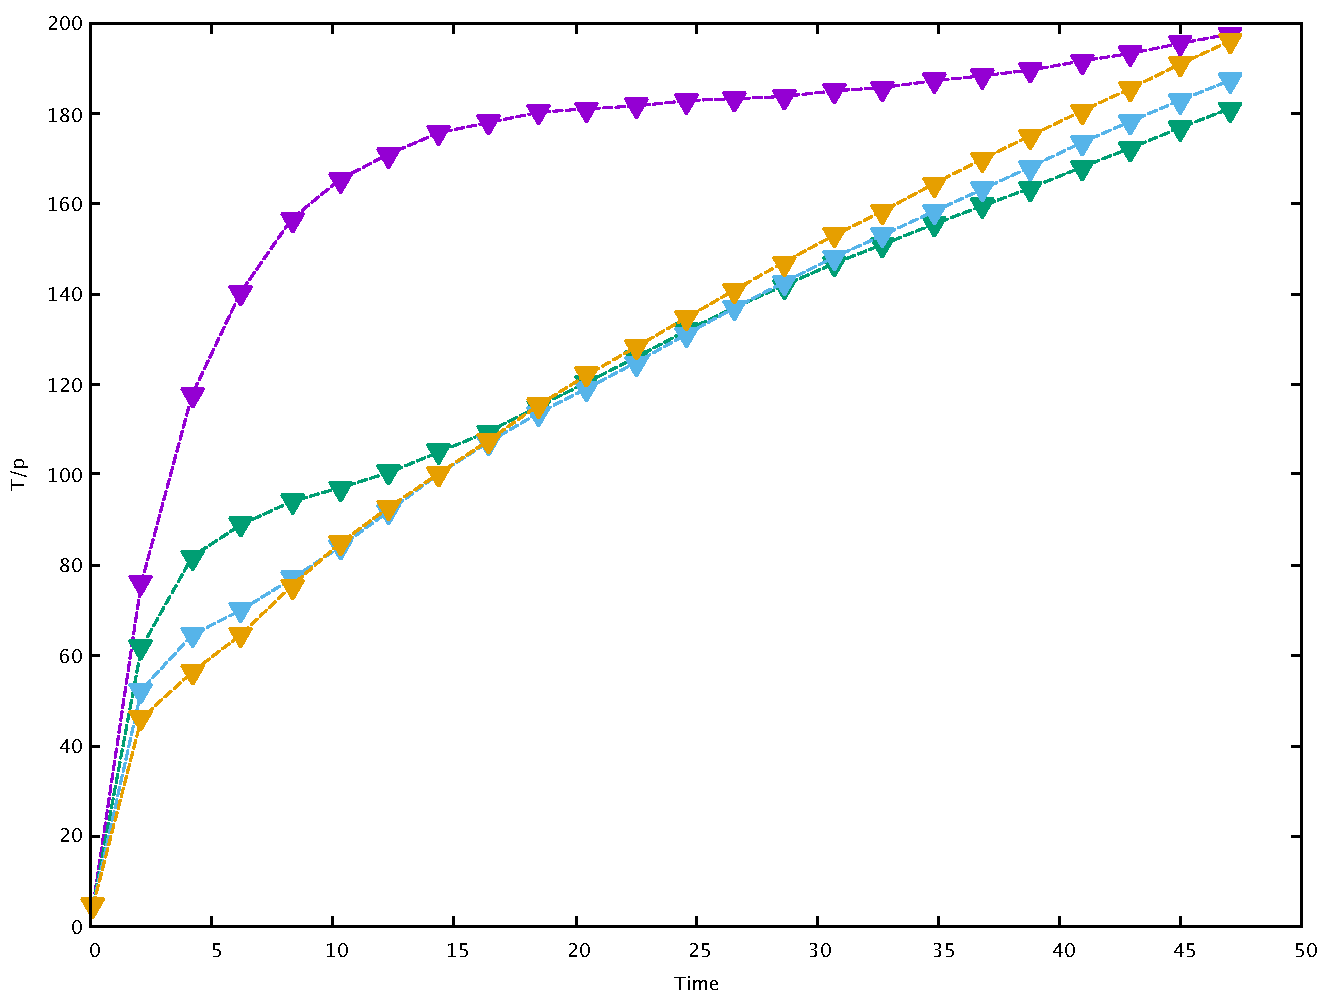
\includegraphics[width=75mm]{./figures/sampled_t_over_p/T_p_lin.pdf} &   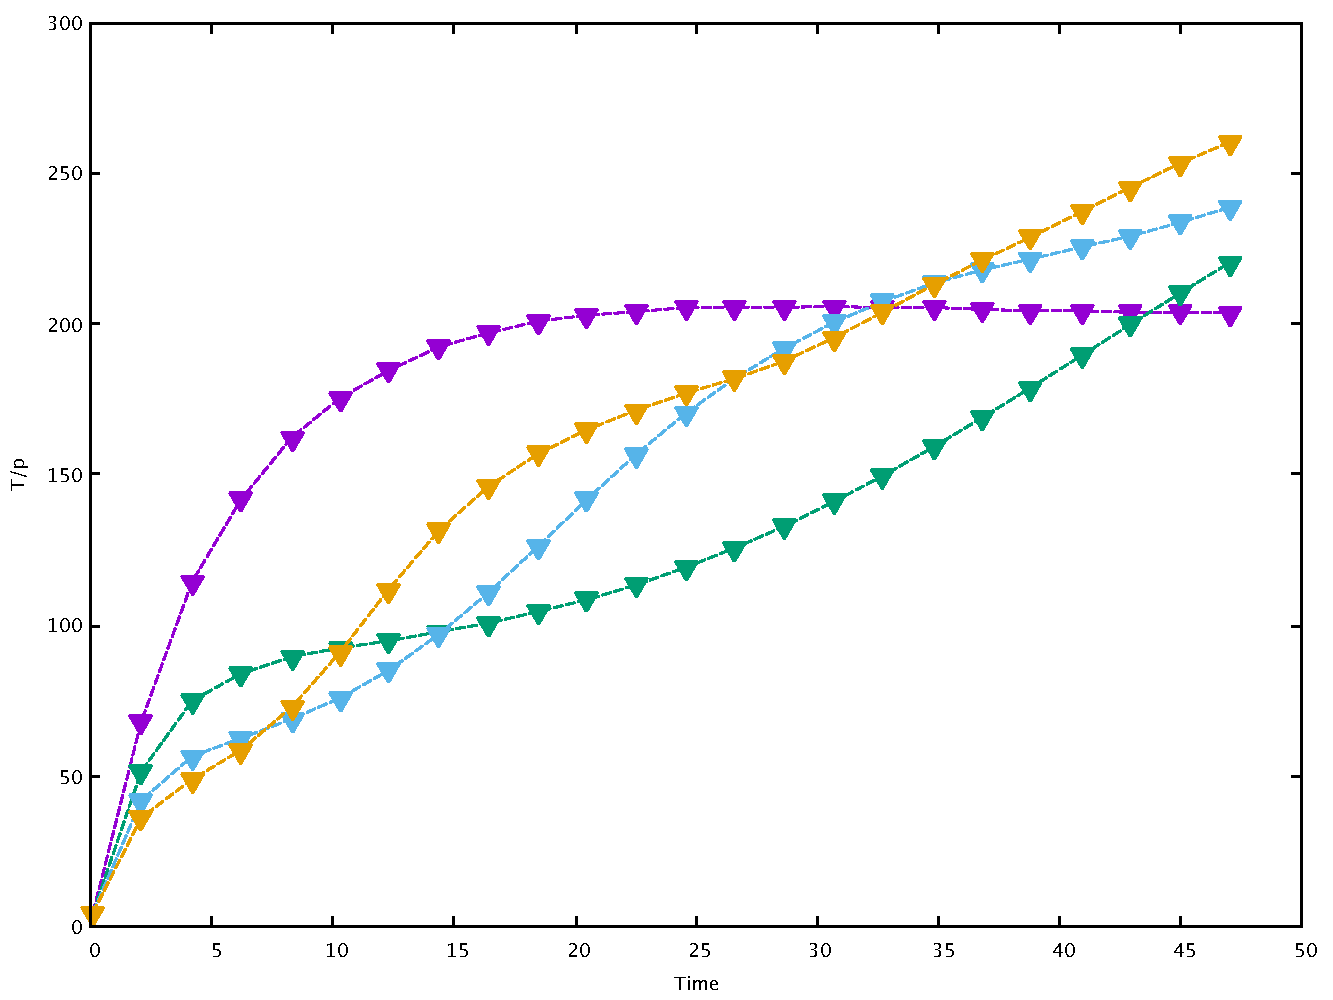
\includegraphics[width=75mm]{./figures/sampled_t_over_p/T_p_cerf.pdf} \\
        (a) lin & (b) Ronald-Cerf\\[6pt]
        \end{tabular}
        \caption[Sampled T/p ]{\textbf{Sampled T/p to show that the min(T/p) will always be the smallest T available.}}
        \end{figure}

        \bpar{\bm{$\min(t_f/p)$}  and run iterations for increasing lower bound \bm{$t_f$}}
         We will begin by studying how the quantity $\min(t_f/p)$ and $iters$ varies with increasing lower bound $t_f^*$.
         In the following plot we show the shape of $t_f/p$ with the time-independent approach and the time-dependent one; for the time being and for sake of semplicity, we consider only the step function Ronald-Cerf(3).
         \begin{figure}[ht]
         \centering
         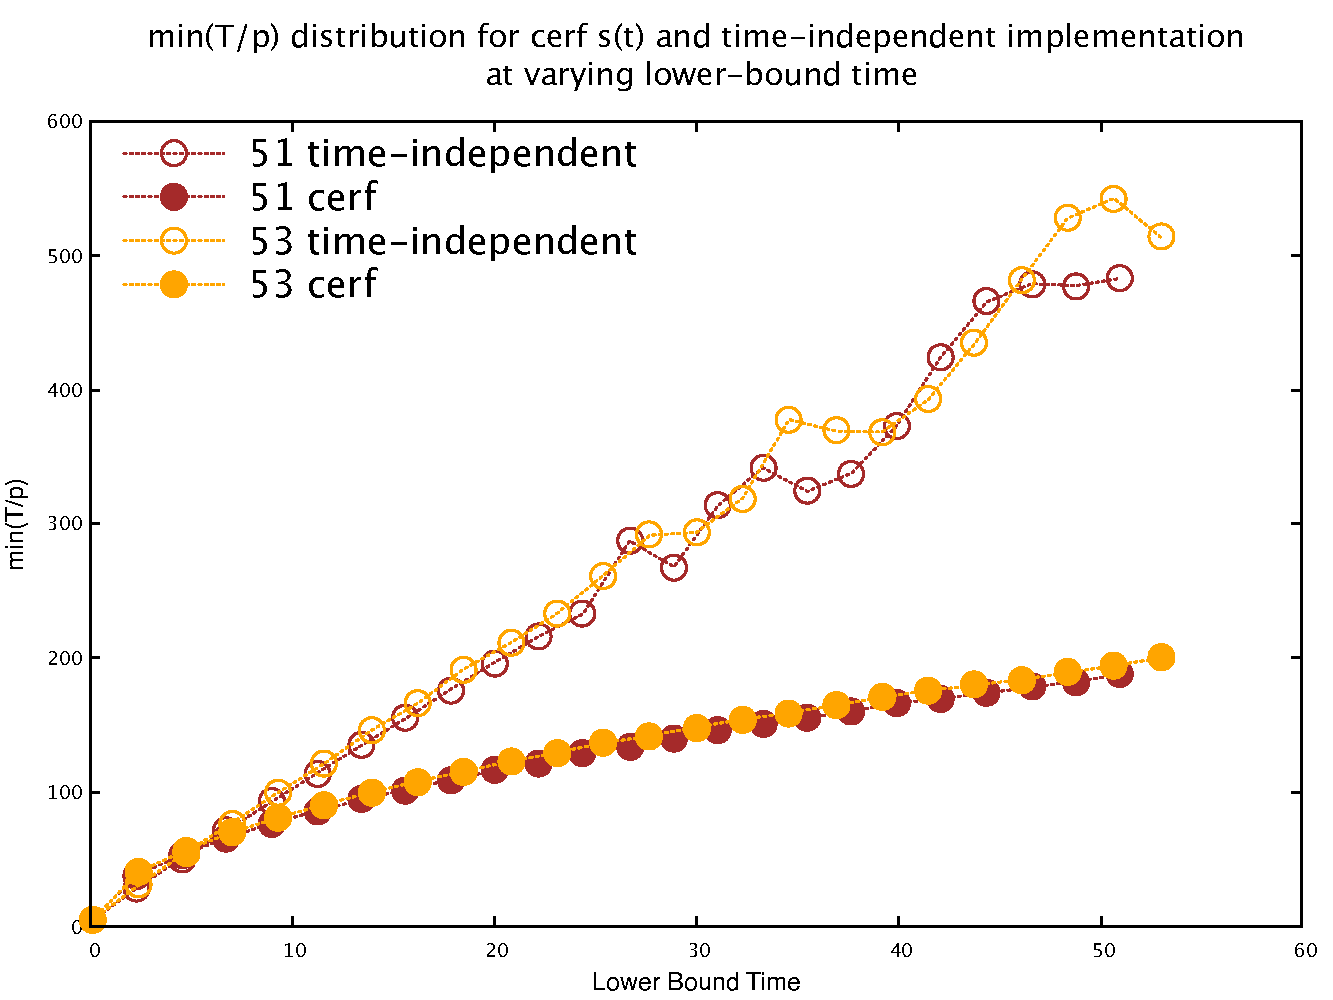
\includegraphics[width=90mm]{./figures/min_tp/delta.pdf}
         \caption[$\min(t_f/P)$ distribution for increasing lower bound time.]{\textbf{\bm{$\min(t_f/P)$} distribution for increasing lower bound time. }The figure shows the distribution of the quantity min(T/p) for increasing values of lower bound time, using the time-independent hamiltonian (circles) and time-dependent hamiltonain (solid circles) and evaluated for a Cy(51) and Cy(53). We see that for times smaller than a characteristic time $T^*$ the time-independent approach performs slightly better, while for large time the time-dependent one performs significantly better. }
         \label{fig:delta_increasing_time}
         \end{figure} \\
        As we can see from the plot the distribution can be diveded into to section marked by a particular $T^*$ (for the time being the value of such time is not of our interest):
        \begin{itemize}
            \item for $t_f<T^*$ the time-independent approach performes slightly better than the time-dependent one.
            \item for $t_f>T^*$ however the time-dependent approach performs significantly better, in particular with increasing time $t_f$
        \end{itemize}
        The behaviour for large T is to be expected, considering that the time-dependent approach shows localization properties and the probability increases with increasing time as we shoed in Figure?, in contrast with the time-independent approach that does not show localization propeties.\\ What this show is that the choice of $t_f$ has great effects on the outcome of our time-dependent approach, making it a successfull or unsuccesfull alternative.
        In terms of iterations the trend is similar to the quantity \quantity, as the following plot shows.
        \begin{figure}[ht]
        \centering
        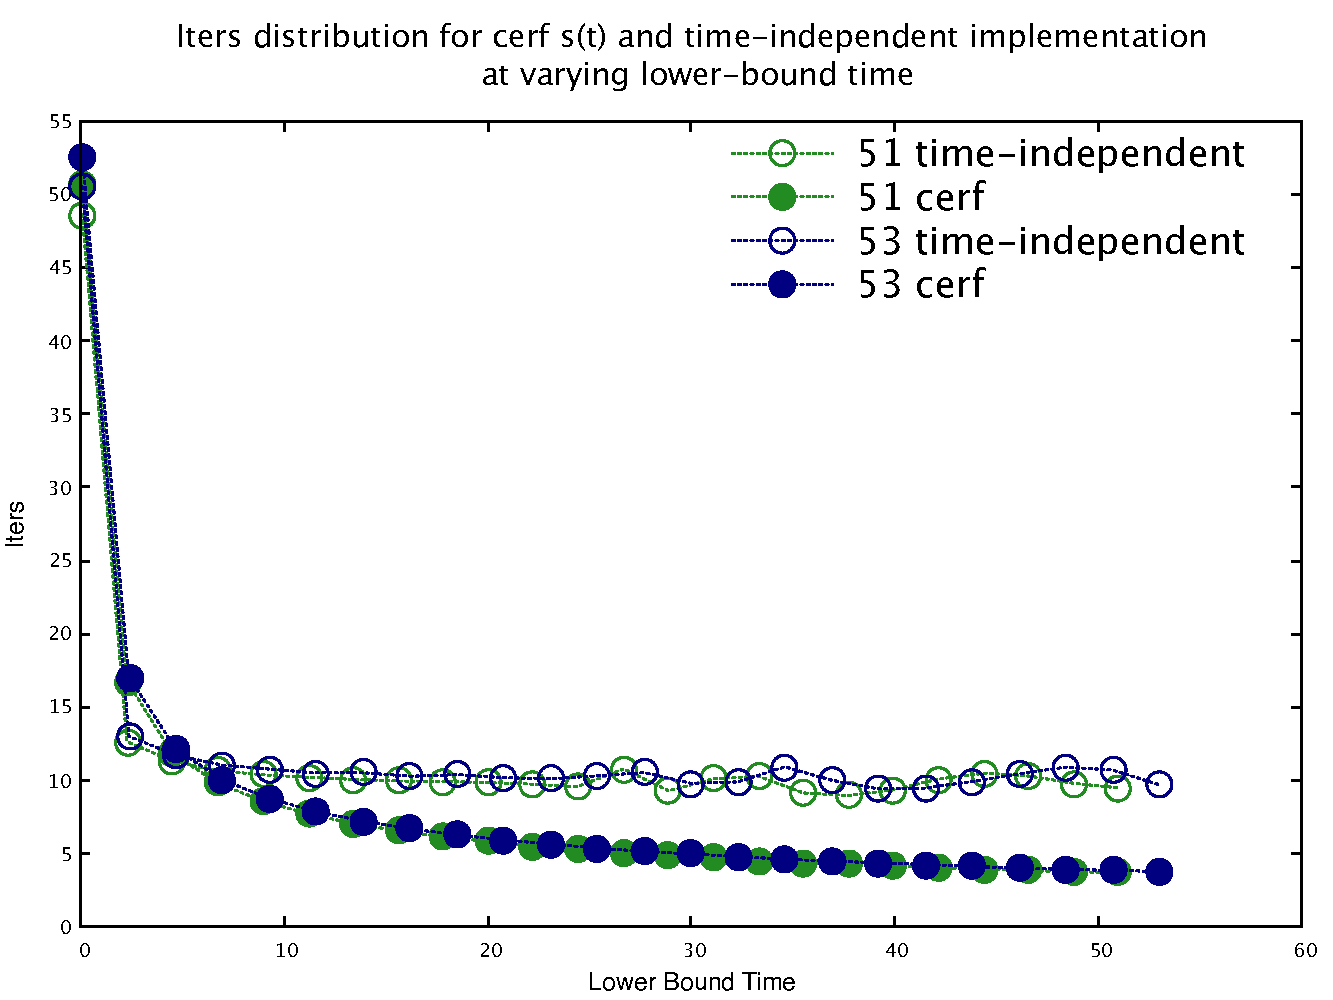
\includegraphics[width=90mm]{./figures/min_tp/iters.pdf}
        \caption[$iters$ distribution for increasing lower bound time.]{\textbf{$\bm{iters}$ distribution for increasing lower bound time. }The figure shows the distribution of $iters$ for increasing values of lower bound time, using the time-independent hamiltonian (circles) and time-dependent hamiltonain (solid circles) and evaluated for a Cy(51) and Cy(53). This distribution reflects the probability distribution of the two approaches: for the time-independent hamiltonian the probability does not increase with time, resulting in a (almost) constant $iters$, while the time-dependent hamiltonian showing localization properties requires less iterations to get to unitary probability.}
        \label{fig:iters_increasing_time}
        \end{figure} \\
        The iterations distribution reflects the overall probability distribution of the time-dependent and time-independent hamiltonian approaches. For small lower bound time the two approaches show a similar performance: the probability is very small, thus requiring a large number of iterations to get to unitary probability. As $t_f$ increases we see two very different trends:
        \begin{itemize}
            \item The time independent approach requires an almost constant number of iterations (the numerical values is somewhat irrelevant since this distribution reflects only the Cy(53) and Cy(55)). This reflects the non-localization properties of this particular approach, for which the probability does not increase with time
            \item On the other hand the time-dependent approach, showing localization properties, requires less iterations to solve the search with unitary probability.
        \end{itemize}
        Taking into account that we're performing a multiple run search and the initialization time $t_{init}$ previously discussed, it is clear that the time-depedent approch performs better than the time-independent counter part in most of the scenario.

        \bpar{\bm{$\min(t_f/p)$} and run iterations with constrained lower bound time}
        In order to show that the lower bound time does indeed have such great impact on the performance of the time-dependen approach relative to the time-independent one we now study the distribution of the quantity $\min(t_f/P)$ with a constrain on the lower bound time. \\ The choice of constrain is arbitrary and somewhat biased since the larger the constrain the better the performance of the time-dependent approach, as we've just shown in \cref{fig:delta_increasing_time}. Therefore, to make the choice fair, we consider the lower bound time to be $t_f^* = \sqrt{N}$ which is the time scaling of the standard Grover's Search, the QW Search on the complete graph and so on. In the best case scenario we discover that the number of iterations necessary to get to unitary probability remain constant regardless of the dimension of the graph, making this approach scale as the ones just mentioned; in the most probable scenario we discover that the number of iterations increase with the graph size, thus adding a scaling factor that depends on some power of N. \\ \\ The following plot shows the distribution of the quantity $\min(t_f/P)$ for circular graphs Cy(N) with N up to 71. The quantity is computed using the time-dependent hamiltonian with linear step function and the time-independent one, with constrained time $t_f=2 \sqrt{N}$
        \begin{figure}[ht]
        \centering
        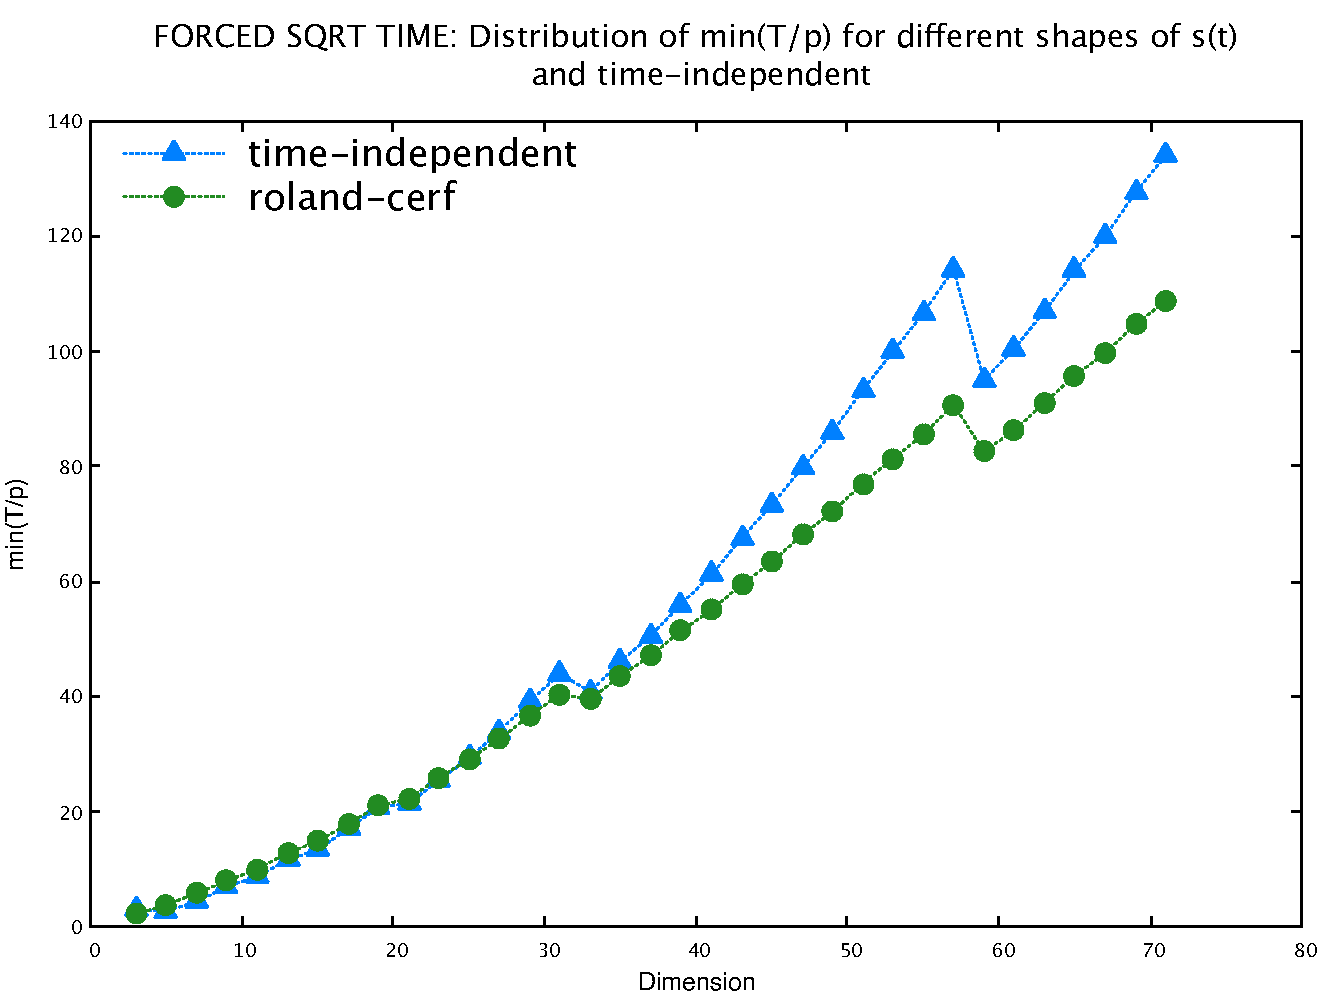
\includegraphics[width=90mm]{./figures/min_tp_sqrt/forced_delta.pdf}
        \caption[$\min(t_f/P)$ distribution for Cy(N) up to N=71 with constrained time at $\sqrt(N)$.]{\textbf{\bm{$\min(t_f/P)$} distribution for Cy(N) up to N=71 with constrained time at $\bm{\sqrt{N}}$.} The figure shows the distribution of the quantity min(T/p) for increasing values of lower bound time, using the time-independent hamiltonian (circles) and time-dependent hamiltonain (solid circles) and evaluated for a Cy(51) and Cy(53). We see that for times smaller than a characteristic time $T^*$ the time-independent approach performs slightly better, while for large time the time-dependent one performs significantly better. }
        \label{fig:delta_increasing_time}
        \end{figure}\\ \\
        \bpar{\bm{$\min(t_f/p)$} and run iterations for different shapes of s(t)}
        We now investigate the effects of the different step functions discussed in section? in the probability distribution and in particular on the quantity $\min(t_f/P)$. As we did for the general time-dependent and time-independent comparison we constrain the lower bound time to be larger than $\sqrt{N}$.
        The following plot shows the distribution of the quantity $\min(t_f/P)$ for circular graphs Cy(N) with N up to 71, using the time-dependent hamiltonian with linear, sqrt, Ronald-Cerf(3) step functions:
        \textbf{include figure}

    \subsection{Comparison: Robustness}
    We now address with a semi-quantitative approach the robustness of the time-dependent and time-independent search. Since we're only interested in the comparison of the two approaches, and not an absolute measure of their robustness, as mentioned in Section? we study the difference of probability for a set perturbance of the $\gamma$ parameter. In particular we investigate for fairly small variation on the parameter (1\%), up to quite large variations (5\% and 10\%). \\ \\We begin by finding the quantity $\min(t_f/P)$ with time constrains ($t_f = \sqrt{N}$). For the corresponding $(t_f,\gamma)$ combination we evaluate the robustness as follows:
    \begin{equation}
        R ^\pm = P(t_f, \gamma) - P(t_f, \gamma \pm \delta\gamma)
    \end{equation}
    where $\delta\gamma$ is the variation of the parameter (1, 5 or 10\% of $\gamma$), that can be both positive and negative. To find a unique value for the robustness an average of $R^\pm$ is done:
    \begin{equation}
        R = \frac{R^++ R^-}{2}
    \end{equation}
    In theory the quantity R should be positive, since the $(t_f,\gamma)$ combination should produce the highest probability possible. The average over positive and negative variations ensure that each approach are treated fairly. \\ \\ For the time-dependent search with only consider the linear step function an the Ronal-Cerf(3). As we showed in the previous section the Ronald-Cerf Hamiltonian performs better than the linear conterpart, while from a qualitative point of view the linear hamiltonian has a smoother probability distribution. The following plots show the semi-quantitative robustness for the $\gamma$ variations in the order of 1\% - 5\% - 10\% for the time-independent search and the time-dependent one with linear and Ronald-Cerf step functions s(t).
    \textbf{Insert figure}



\section{Results for the Complete Graph}
    \subsection{Search results from Wong(2016)}
    \subsection{Localization results}
